%%%%%%%%%%%%%%%%%%%%%%%%%%%%%%%%%%%%%%%%%%%%%%%%%%%%%%%%%%%%%%%%%%%%%%%%%%%%%%%%
%2345678901234567890123456789012345678901234567890123456789012345678901234567890
%        1         2         3         4         5         6         7         8

\documentclass[letterpaper, 10 pt, journal]{ieeeconf}  % Comment this line out if you need a4paper

%\documentclass[a4paper, 10pt, conference]{ieeeconf}      % Use this line for a4 paper

\IEEEoverridecommandlockouts                              % This command is only needed if 
                                                          % you want to use the \thanks command

\overrideIEEEmargins                                      % Needed to meet printer requirements.

% See the \addtolength command later in the file to balance the column lengths
% on the last page of the document

% The following packages can be found on http:\\www.ctan.org
%\usepackage{graphics} % for pdf, bitmapped graphics files
%\usepackage{epsfig} % for postscript graphics files
%\usepackage{mathptmx} % assumes new font selection scheme installed
%\usepackage{times} % assumes new font selection scheme installed
%\usepackage{amsmath} % assumes amsmath package installed
%\usepackage{amssymb}  % assumes amsmath package installed
\usepackage{graphicx}
\usepackage{cite}
\setlength{\textheight}{9.4in}

\title{\LARGE \bf
Evo-ROS: Integrating Evolutionary Robotics and ROS*
}


\author{Jared Moore,$^{1}$ Anthony Clark,$^{2}$ Glen Simon$^{3}$ and Philip McKinley$^{3}$% <-this % stops a space
\thanks{*This work was supported by the U.S. Air Force Research Laboratory.}% <-this % stops a space
\thanks{$^{1}$School of Computing and Information Systems, Grand Valley State University, USA}
\thanks{$^{2}$Department of Computer Science, Missouri State University, USA}
\thanks{$^{3}$Department of Computer Science and Engineering, Michigan State University, USA}
}

%% 
%% \author[1]{Jared Moore}
%% \author[2]{Anthony Clark}
%% \author[3]{Glen Simon}
%% \author[3]{Philip McKinley}
%% \affil[1]{\small School of Computing and Information Systems, Grand Valley State University, USA}
%% \affil[2]{Department of Computer Science, Missouri State University, USA}
%% \affil[3]{Department of Computer Science and Engineering, Michigan State University, USA}
%% 

\begin{document}

\newcommand{\project}{Evo-ROS}


\maketitle

\thispagestyle{empty}
\pagestyle{empty}


%%%%%%%%%%%%%%%%%%%%%%%%%%%%%%%%%%%%%%%%%%%%%%%%%%%%%%%%%%%%%%%%%%%%%%%%%%%%%%%%
\begin{abstract}

We introduce Evo-ROS, a framework combining evolutionary search
and ROS/Gazebo-based simulation. The framework 
enables researchers and developers to take
advantage of evolutionary search during design. 
Evolutionary algorithms can be applied to many aspects of 
robot development,
including optimal configuration and placement of sensors and
actuators, generation of compensatory behavior in case of
failed/faulty components, and detection of
“unlikely-but-possible” situations that might cause system failure.  
\end{abstract}


%%%%%%%%%%%%%%%%%%%%%%%%%%%%%%%%%%%%%%%%%%%%%%%%%%%%%%%%%%%%%%%%%%%%%%%%%%%%%%%%
\vspace{-0.1in}
\section{MOTIVATIONS}

Evolutionary robotics (ER)~\cite{Floreano2008} applies the basic principles of genetic evolution to the design of robots through the application of the genetic algorithm~(GA).
%
An artificial genome specifies the robot's control system and possibly aspects of its morphology~(body).
%
Individuals in a population are evaluated~(typically in simulation) with respect to one or more tasks, with the best performing individuals selected to pass their genes to the next generation.
%
Evolutionary approaches have yielded effective controllers and physical designs for a variety of 
walking, swimming, and flying robots, e.g.,~\cite{Floreano2008,Clark.JournalBB.2015,MooreALIFEJournal}.
%
% Our own research has applied evolutionary algorithms to optimize both morphology and control
% in aquatic and terrestrial robots~\cite{Clark.JournalBB.2015,MooreALIFEJournal}.  
%
% Evolving robot behavior and morphology is interesting in its own right, but 
An advantage of evolutionary search is the possible discovery of solutions (as well as potential problems) that the engineer might not otherwise have considered.

Simulation is an essential component of 
evolutionary robotics, greatly reducing the 
time to evolve solutions while avoiding possible damage to physical robots.
%
However, the ER community generally does not take advantage of complex tools
used in mainstream robotics, such as the Robot Operating System (ROS).
% , Gazebo simulator, and autopilot software such as Ardupilot.
% By providing tested models of commercially available hardware, ROS/Gazebo provides a platform to study high-level behaviors while saving developer time during the design phase.  
% %
% Additionally, results have been shown to transfer to real robots, potentially addressing the ``reality-gap'' often encountered in ER~\cite{Koos2010}.  
In turn, use of evolutionary algorithms is not widespread in mainstream robotics.


\section{DESIGN}
To help address both issues, we have developed an evolutionary framework, {\project}, that integrates ROS-based simulations for robot evaluation.  
%
Our current prototype includes ROS coupled with the Gazebo simulator, along
with Ardupilot, open-source software/firmware supporting a
variety of autopilot hardware and autonomous vehicles.

A GA or other evolutionary algorithm is configured as a
front-end, handling the details of genomes, populations, and
selection, with ROS-based simulations invoked to evaluate
individual robots or possibly groups of collaborating robots.
The GA sends genomes to a ROS/Gazebo instance via sockets.
After evaluation, a 
fitness score is returned through another socket.
%
In comparison to a typical ROS/Gazebo simulation, the primary extension a user needs to implement is mapping a genome into the robotic system.  
%
As a proof-of-concept, we have 
used Evo-ROS to enhance LIDAR-based obstacle avoidance and navigation in 
Erle-Rover, a commercial terrestrial robot; see Figure~\ref{f:erlerover}.


%
Although individual simulations in ROS/Gazebo often require substantially more wall-clock time than those of typical ER  simulators, 
%
evaluations are ``pleasantly parallel'' and can be 
distributed across computing resources to speed up the execution time for each generation.  
%
Depending on the specific plugin stack required, one ROS instance can spawn 
multiple Gazebo instances, or single ROS/Gazebo pairs can be distributed across multiple virtual machines~(VMs).  
%
We have tested both approaches.

\begin{figure}[htb]
\centering
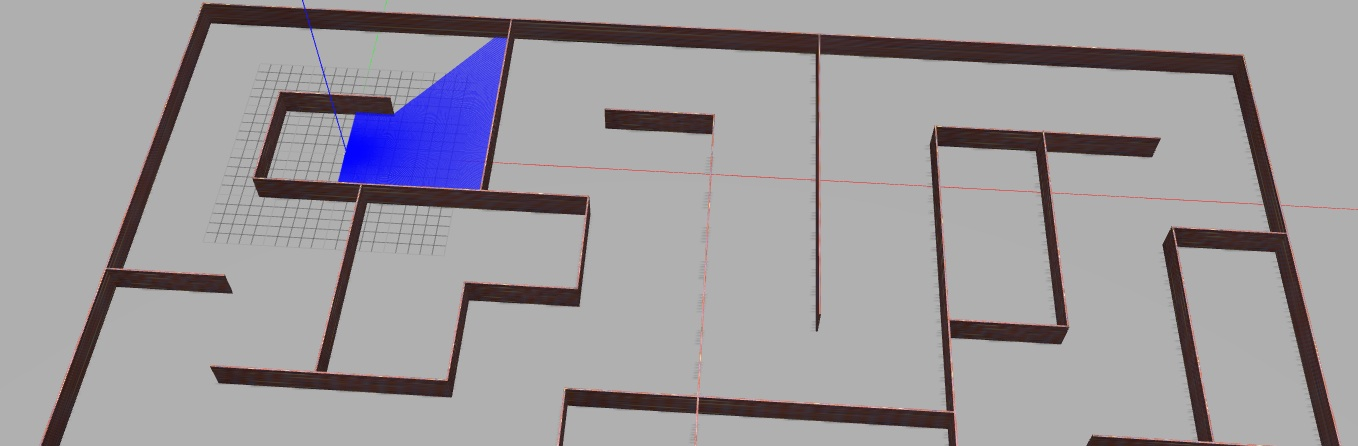
\includegraphics[width=2.8in]{rover_maze_2-crop1.jpg}

\vspace{0.1in}
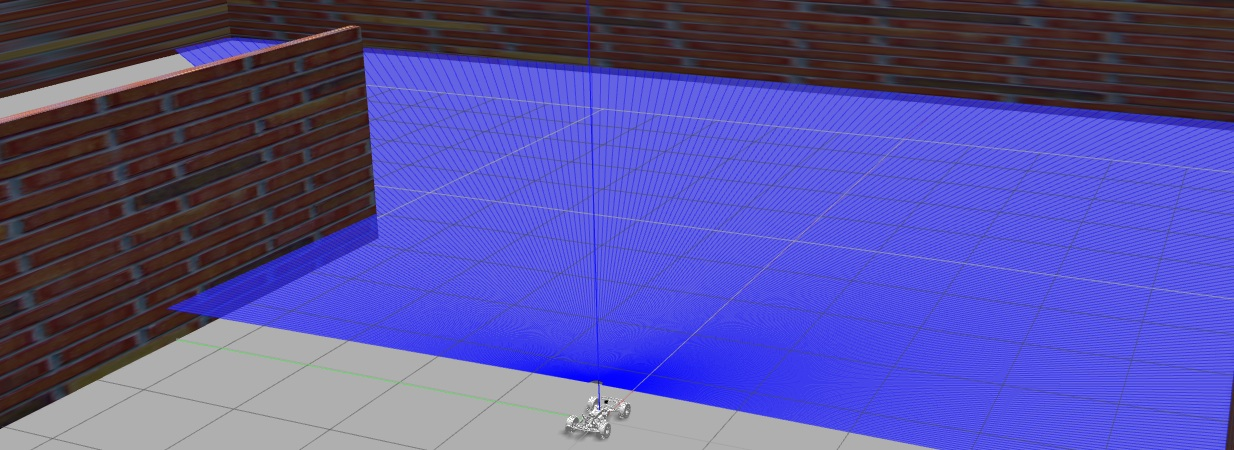
\includegraphics[width=2.8in]{rover_maze_1-crop2.jpg}
\caption{Wide-angle (top) and close-up (bottom) of simulated Erle-Rover terrestrial robot with evolved LIDAR-related parameters navigating a maze.}
\label{f:erlerover}
\end{figure}

\vspace{-0.2in}
\section{CONCLUSIONS}
Evo-ROS is intended to provide the robotics community with a new tool to aid in robot design and testing.
%
Although thus far we have focused on terrestrial robots, the integration of Ardupilot means {\project} can be directly applied to a variety of other autonomous vehicles, including copters and planes.
Source code and examples are available at: https://github.com/jaredmoore/EvoROS.
%

\begin{small}
\bibliographystyle{IEEEtran}
% \bibliographystyle{ieeetr}
%\clearpage
\bibliography{References/pubs2011-present,References/references}
\end{small}



\end{document}
